% // ============================================================================
%//
%// Copyright (c) 1999 The CGAL Consortium
%//
%// This software and related documentation is part of an INTERNAL release
%// of the Computational Geometry Algorithms Library (CGAL). It is not
%// intended for general use.
%//
%// ----------------------------------------------------------------------------
%//
%// release       :
%// release_date  :
%//
%// file          : /doc_tex/basic/Triangulation3/Triangulation3.tex
%// revision      : $Revision$
%//
%// author(s)     : Monique Teillaud <Monique.Teillaud@sophia.inria.fr>
%//
%// coordinator   : INRIA Sophia Antipolis (Mariette Yvinec <Mariette.Yvinec@sophia.inria.fr>)
%//
%//============================================================================
\chapter{3D Triangulations}
\label{chapter-Triangulation3}

\vspace*{-1cm}
\minitoc

\begin{ccTexOnly}
%\vspace*{-1cm}
\begin{center}
\includegraphics[width=6cm]{grid.eps} \hspace*{2cm} 
\includegraphics[width=6cm]{sphere.eps} 
\end{center}
\end{ccTexOnly}
\begin{ccHtmlOnly}
<img border=0 src="./sphere.gif" align=center>
<img border=0 src="./grid.gif" align=center>
\end{ccHtmlOnly}

The basic 3D-triangulation class of \cgal\ is primarily designed to
represent the triangulations of a set of points $A$ in $\R^3$.  It is
a partition of the convex hull of {$A$} into tetrahedra whose vertices
are the points of {$A$}.  Together with the unbounded cell having the
convex hull boundary as its frontier, the triangulation forms a
partition of $\R^3$. Its cells ($3$-faces) are such that two cells
either do not intersect or share a common facet ($2$-face), edge
($1$-face) or vertex ($0$-face).

\section{Representation}
\label{Triangulation3-sec-intro}

In order to deal
only with tetrahedra, which is convenient for many applications, the
unbounded cell can be subdivided into tetrahedra by considering that
each convex hull facet is incident to an \ccc{infinite cell} having as
fourth vertex an auxiliary vertex called the \ccc{infinite vertex}.  In
that way, each facet is incident to exactly two cells and special cases
at the boundary of the convex hull are simple to deal with.

The class \ccc{Triangulation_3<TriangulationTraits_3,TriangulationDataStructure_3>} of \cgal\ implements this
point of view and therefore considers the triangulation of the set
of points as a set of finite and infinite tetrahedra.  Notice that the
infinite vertex has no significant coordinates and that no
geometric predicate can be applied on it.

A triangulation is a collection of vertices and cells that are linked
together through incidence and adjacency relations. Each cell gives
access to its four incident vertices and to its four adjacent
cells. Each vertex gives access to one of its incident cells.

The four vertices of a cell are indexed with 0, 1, 2 and 3 in positive
orientation, the positive orientation being defined by the orientation
of the underlying Euclidean space $\R^3$. The neighbors of a cell are also
indexed with 0, 1, 2, 3 in such a way that the neighbor indexed by $i$
is opposite to the vertex with the same index. See
Figure~\ref{Triangulation3-fig-orient}.

\begin{figure}[htbp]
\begin{ccTexOnly}
\begin{center} 
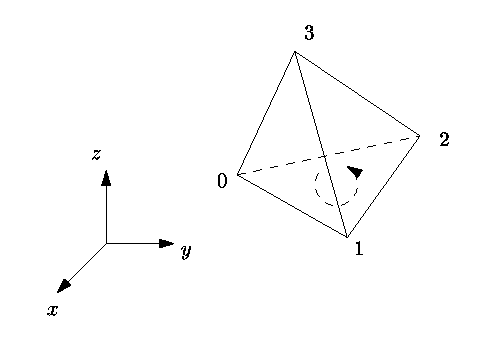
\includegraphics{orient.eps} 
\end{center}
\end{ccTexOnly}
\caption{Orientation of a cell (3-dimensional case).
\label{Triangulation3-fig-orient}}
\begin{ccHtmlOnly}
<CENTER>
<img border=0 src="./orient.gif" align=center alt="Orientation of a cell 
(3-dimensional case)">
</CENTER>
\end{ccHtmlOnly}
\end{figure} 

As in the underlying combinatorial triangulation (see
Chapter~\ref{chapter-TDS3}), edges ($1$-faces) and facets ($2$-faces)
are not explicitly 
represented: a facet is given by a cell and an index (the facet
\ccc{i} of a cell \ccc{c} is the facet of \ccc{c} that is opposite to
the vertex with index \ccc{i}) and an edge is given by a cell and two
indices (the edge \ccc{(i,j)} of a cell \ccc{c} is the edge whose
endpoints are the vertices of \ccc{c} with indices \ccc{i} and
\ccc{j}). See Figure~\ref{TDS3-fig-repres}.  

\paragraph{Degenerate Dimensions}
The class \ccc{Triangulation_3} can also deal with
triangulations whose dimension is less than~3. A triangulation of a
set of points in $\R^d$ covers the whole space $\R^d$ and consists of
cells having $d+1$ vertices: some of them are infinite, they are
obtained by linking the additional infinite vertex to each facet of
the convex hull of the points.
\begin{itemize}
\item {} \emph{dimension 2:} when a triangulation only contains
coplanar points (which is the case when there are only three points), 
it consists of triangular faces.
\item {} \emph{dimension 1:} the triangulation contains only collinear 
points (which is the case when there are only two points), it consists
of edges.
\item {} \emph{dimension 0:} the triangulation contains only one
finite point.
\item {} \emph{dimension -1:} this is a convention to handle the case
when the only vertex of the triangulation is the infinite one.
\end{itemize} 

The same cell class is used in all cases: triangular faces in
2D can be considered as degenerate cells, having only three vertices
(resp. neighbors) numbered $(0,1,2)$;
edges in 1D have only two vertices (resp. neighbors) numbered $0$ and $1$. 

The implicit representation of facets (resp. edges) still holds
for degenerate dimensions (\textit{i.e.} dimensions $<3$) : in
dimension~2, each cell has only one facet of index 3, and 3 edges
$(0,1)$, $(1,2)$ and $(2,0)$; in dimension~1, each cell has one edge
$(0,1)$.  

\paragraph{Validity}
A triangulation of $\R^3$ is said to be \ccc{locally valid} iff

{\bf (a)-(b)} Its underlying combinatorial graph, the triangulation
data structure, is \ccc{locally valid} 
(see Section~\ref{TDS3-sec-intro} of Chapter~\ref{chapter-TDS3})\\
{\bf (c)} Any cell has its vertices ordered according to positive
orientation. See Figure~\ref{Triangulation3-fig-orient}.

When the triangulation is degenerated into a triangulation of
dimension~2, the  geometric validity reduces to:

{\bf (c-2D)} For any two adjacent triangles $(u,v,w_1)$ and $(u,v,w_2)$ with
common edge $(u,v)$, $w_1$ and $w_2$ lie on opposite sides of $(u,v)$
in the plane.

When all the points are collinear, this condition becomes:

{\bf (c-1D)} For any two adjacent edges $(u,v)$ and $(v,w)$, $u$ and
$w$ lie on opposite sides of the common vertex $v$ on the line.

The \ccc{is_valid()} method provided in \ccc{Triangulation_3} checks
the local validity of a given triangulation. This does not always
ensure global validity \cite{mnssssu-cgpvg-96,dlpt-ccpps-98} but it is 
sufficient for practical cases.


\section{Delaunay Triangulation} 

The class \ccc{Delaunay_triangulation_3} represents a three-dimensional
Delaunay triangulation.

Delaunay triangulations have the specific \textit{empty sphere property},
that is, the circumscribing sphere of each cell of such a triangulation
does not contain any other vertex of the triangulation in its interior.
These triangulations are uniquely defined except in degenerate cases
where five points are cospherical.  Note however that the \cgal\ implementation
computes a unique triangulation even in these cases.

This implementation is fully dynamic: it supports both insertions of points
and vertex removal.
The user is advised to use the class \ccc{Triangulation_hierarchy_3} in
order to benefit from an increased efficiency for large data sets. 

\section{Regular Triangulation} 
\label{Triangulation3-sec-class-Regulartriangulation}

The class \ccc{Regular_triangulation_3} implements incremental regular
triangulations, also known as weighted Delaunay triangulations.

Let ${S}^{(w)}$ be a set of weighted points in $\R^3$. Let
${p}^{(w)}=(p,w_p), p\in\R^3, w_p\in\R$ and 
${z}^{(w)}=(z,w_z), z\in\R^3, w_z\in\R$ be two weighted points. 
A weighted point
${p}^{(w)}=(p,w_p)$ can also be seen as a sphere of center $p$ and
radius $w_p$. 
The \textit{power product} between ${p}^{(w)}$ and ${z}^{(w)}$ is
defined as 
\[\Pi({p}^{(w)},{z}^{(w)}) = {\|{p-z}\|^2-w_p-w_z}\]
where $\|{p-z}\|$ is the Euclidean distance between $p$ and $z$. 
 ${p}^{(w)}$ and ${z}^{(w)}$
are said to be \textit{orthogonal} iff $\Pi{({p}^{(w)},{z}^{(w)})}
= 0$ (see Figure~\ref{Triangulation3-fig-ortho}).

\begin{figure}[htbp]
\begin{ccTexOnly}
\begin{center} 
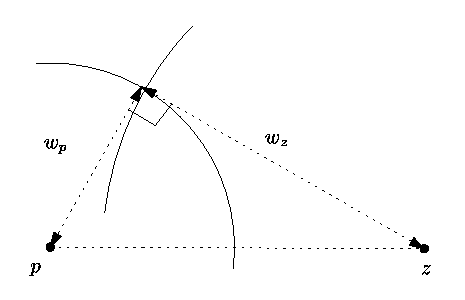
\includegraphics{ortho.eps} 
\end{center}
\end{ccTexOnly}
\caption{Orthogonal weighted points (picture in 2D).
\label{Triangulation3-fig-ortho}}
\begin{ccHtmlOnly}
<CENTER>
<img border=0 src="./ortho.gif" align=center alt="Orthogonal weighted
points (picture in 2D)"> 
</CENTER>
\end{ccHtmlOnly}
\end{figure} 

Four weighted points have a unique common orthogonal weighted point
called the \textit{power sphere}.  The weighted point orthogonal to
three weighted points in the plane defined by these three points is
called the \textit{power circle}. The
\textit{power segment} will denote the weighted point orthogonal to
two weighted points on the line defined by these two points.

A sphere ${z}^{(w)}$ is said to be
\textit{regular} if $\forall {p}^{(w)}\in{S}^{(w)},
\Pi{({p}^{(w)},{z}^{(w)})}\geq 0$.

A triangulation of ${S}^{(w)}$ is \textit{regular} if the power spheres
of all simplices are regular. 

The regular triangulation of
${S}^{(w)}$ is in fact the projection onto $\R^3$ of the convex hull 
of the four-dimensional points $(p,\|p-O\|^2-w_p),$ for
${p}^{(w)}=(p,w_p)\in{S}^{(w)}$. 
Note that all points of ${S}^{(w)}$ do not
necessarily appear as vertices of the regular
triangulation. To know more about regular triangulations, see for
example \cite{es-itfwr-96}. 

When all weights are 0, power spheres are nothing more than
circumscribing spheres, and the regular triangulation is exactly the
Delaunay triangulation.

\section{Triangulation hierarchy} 

The class \ccc{Triangulation_hierarchy_3} implements a
triangulation augmented with a data structure that allows fast point
location queries. Thus, it allows fast construction of the
triangulation. As proved in~\cite{d-dh-02}, this structure has an
optimal behavior when it is built for Delaunay triangulations.

Note that, since the algorithms that are provided are randomized, the
running time of constructing a triangulation with a hierarchy may be
improved when shuffling the data points.

\section{Software Design}
\label{Triangulation3-sec-design}

The main classes \ccc{Triangulation_3}, \ccc{Delaunay_triangulation_3} and
\ccc{Regular_triangulation_3} are connected to each other by the
derivation diagram shown in Figure~\ref{t3_derivation}.  This diagram
also shows two other classes: \ccc{Triangulation_utils_3}\lcTex{
(\ccRefPage{CGAL::Triangulation_utils_3})}, which provides
a set of tools operating on the indices of vertices in cells,
and \ccc{Triangulation_hierarchy_3}, which implements a hierarchy of
triangulations suitable for speeding up point location.

\begin{figure}[htbp]
\begin{ccTexOnly}
\begin{center} 
\includegraphics{derivation.eps} 
\end{center}
\end{ccTexOnly}
\caption{Derivation diagram of the 3D triangulation classes.
\label{t3_derivation}}
\begin{ccHtmlOnly}
<CENTER>
<img border=0 src="./derivation.gif" align=center
 alt="Derivation diagram of the 3D triangulation classes"> 
</CENTER>
\end{ccHtmlOnly}
\end{figure} 

The three main classes (\ccc{Triangulation_3}, \ccc{Delaunay_triangulation_3}
and \ccc{Regular_triangulation_3}) provide high-level geometric functionality
such as location of a point in the triangulation~\cite{dpt-wt-02}, insertion
and possibly removal of a point~\cite{dt-pvr3d-03}, and are responsible for the
geometric validity.  They are built as layers on top of a triangulation data
structure, which stores their combinatorial structure.  This separation between
the geometry and the combinatorics is reflected in the software design by the
fact that these three triangulation classes take two template parameters :

\begin{itemize}
\item {} the \textbf{geometric traits} class, which provides the type of points
to use as well as the elementary operations on them (predicates and
constructions).  The concepts for these parameters are described in more
details in Section~\ref{Triangulation3-sec-Traits}\lcTex{ and in 
\ccRefPage{TriangulationTraits_3}}.
\item {} the \textbf{triangulation data structure} class, which stores their
combinatorial structure, described in Section~\ref{TDS3-sec-design} of
Chapter~\ref{chapter-TDS3}.
\end{itemize}

The class \ccc{Triangulation_hierarchy_3} is parameterized by a class, which at
the moment can only be \ccc{Delaunay_triangulation_3}.  It fetches its
geometric traits from this parameter directly.

\subsection{The Geometric Traits Parameter}
\label{Triangulation3-sec-Traits}

The first template parameter of the triangulation class
\ccc{Triangulation_3<TriangulationTraits_3, TriangulationDataStructure_3>}
is the geometric traits class, described by the concept
\ccc{TriangulationTraits_3}.  It must define the types of the geometric objects
(points, segments, triangles and tetrahedra) forming the triangulation together
with a few geometric predicates on these objects: orientation in space,
orientation in case of coplanar points, order of collinear points.

In addition to the requirements described before, the geometric traits
class of \ccc{Delaunay_triangulation_3} must define predicates to test for the
\textit{empty sphere property}.  It is described by the concept
\ccc{DelaunayTriangulationTraits_3}, which refines \ccc{TriangulationTraits_3}.

The kernels provided by CGAL: \ccc{Cartesian}, \ccc{Homogeneous},
\ccc{Simple_cartesian}, \ccc{Simple_homogeneous} and
\ccc{Filtered_kernel} can all be used as models for the geometric traits
parameter.
They supply the user with all the functionalities described for the concepts
\ccc{TriangulationTraits_3}\lcTex{
(\ccRefPage{TriangulationTraits_3})} and
\ccc{DelaunayTriangulationTraits_3}\lcTex{
(\ccRefPage{DelaunayTriangulationTraits_3})}.
In addition, the predefined kernels
\ccc{Exact_predicates_inexact_constructions_kernel}\lcTex{
(\ccRefPage{Exact_predicates_inexact_constructions_kernel})} and
\ccc{Exact_predicates_exact_constructions_kernel}\lcTex{
(\ccRefPage{Exact_predicates_exact_constructions_kernel})}
can also be used, the later being recommended when the dual construction is
used.

In order to be used as the traits class for \ccc{Regular_triangulation_3},
a class must provide functions to compute the \textit{power tests}.
(See Section~\ref{Triangulation3-sec-class-Regulartriangulation}.)
\ccc{Regular_triangulation_euclidean_traits_3<R,Weight>} is a traits class 
 designed to be used by the class
\ccc{Regular_triangulation_3<RegularTriangulationTraits_3, TriangulationDataStructure_3>}. It provides
\ccc{Weighted_point}, a class for weighted points
needed by the regular triangulation, which derives from the three dimensional
point class \ccc{R::Point_3}.
It supplies the user with all the functionalities 
described for the concept \ccc{RegularTriangulationTraits_3}\lcTex{
(\ccRefPage{RegularTriangulationTraits_3})}. 
It can be used as a traits class for
\ccc{Regular_triangulation_3<RegularTriangulationTraits_3,
TriangulationDataStructure_3>}.

\subsection{The Triangulation Data Structure Parameter}
\label{Triangulation3-sec-tds}

The second template parameter of the main classes (\ccc{Triangulation_3},
\ccc{Delaunay_triangulation_3} and \ccc{Regular_triangulation_3}) is a
triangulation data structure class.  This class can be seen as a container for
the cells and vertices maintaining incidence and adjacency relations (see
Chapter~\ref{chapter-TDS3}).  A model of this triangulation data structure is
\ccc{Triangulation_data_structure_3}\lcTex{
(\ccRefPage{CGAL::Triangulation_data_structure_3<TriangulationDSVertexBase_3,TriangulationDSCellBase_3>})},
and it is described by the \ccc{TriangulationDataStructure_3} concept
\lcTex{(\ccRefPage{TriangulationDataStructure_3})}.  This model is itself
parameterized by a vertex base and a cell base classes, which gives the
possibility to customize the vertices and cells used by the triangulation data
structure, and hence by the geometric triangulation using it.  Depending on the
kind of triangulation used, the requirements on the vertex and cell base
classes vary, and are expressed by various concepts, following the refinement
diagram shown in Figure~\ref{T3-concept-hierarchy}.

\begin{figure}[htbp]
\begin{ccTexOnly}
\begin{center}
\includegraphics[width=13cm]{concept_hierarchy.eps}
\end{center}
\end{ccTexOnly}
\caption{Concepts refinement hierarchy for the vertex and cell base classes
parameters.
\label{T3-concept-hierarchy}}
\begin{ccHtmlOnly}
<CENTER>
<img border=0 src="./concept_hierarchy.gif" align=center
 alt="Concepts refinement hierarchy for the vertex and cell base classes
parameters.">
</CENTER>
\end{ccHtmlOnly}
\end{figure}

A default value for the triangulation data structure parameter is provided in
all the triangulation classes, so it need not be specified by the user unless
he wants to use a different triangulation data structure or a different vertex
or cell base class.

\subsection{Flexibility of the Design}

In order to satisfy as many uses as possible, a design has been selected that
allows to exchange different parts to meet the users' needs, while still
re-using a maximum of the provided functionalities.  We have already seen that
the main triangulation classes are parameterized by a geometric traits class
and a triangulation data structure (TDS), so that each of them can be
interchanged with alternate implementations.

The most useful flexibility is the ability given to the user to add his own
data in the vertices and cells by providing his own vertex and cell base
classes to \ccc{Triangulation_data_structure_3}.  The
Figure~\ref{T3-fig-layers} shows in more detail the flexibility that is
provided, and the place where the user can insert his own vertex and/or cell
base classes.

\begin{figure}[htbp]
\begin{ccTexOnly}
\begin{center}
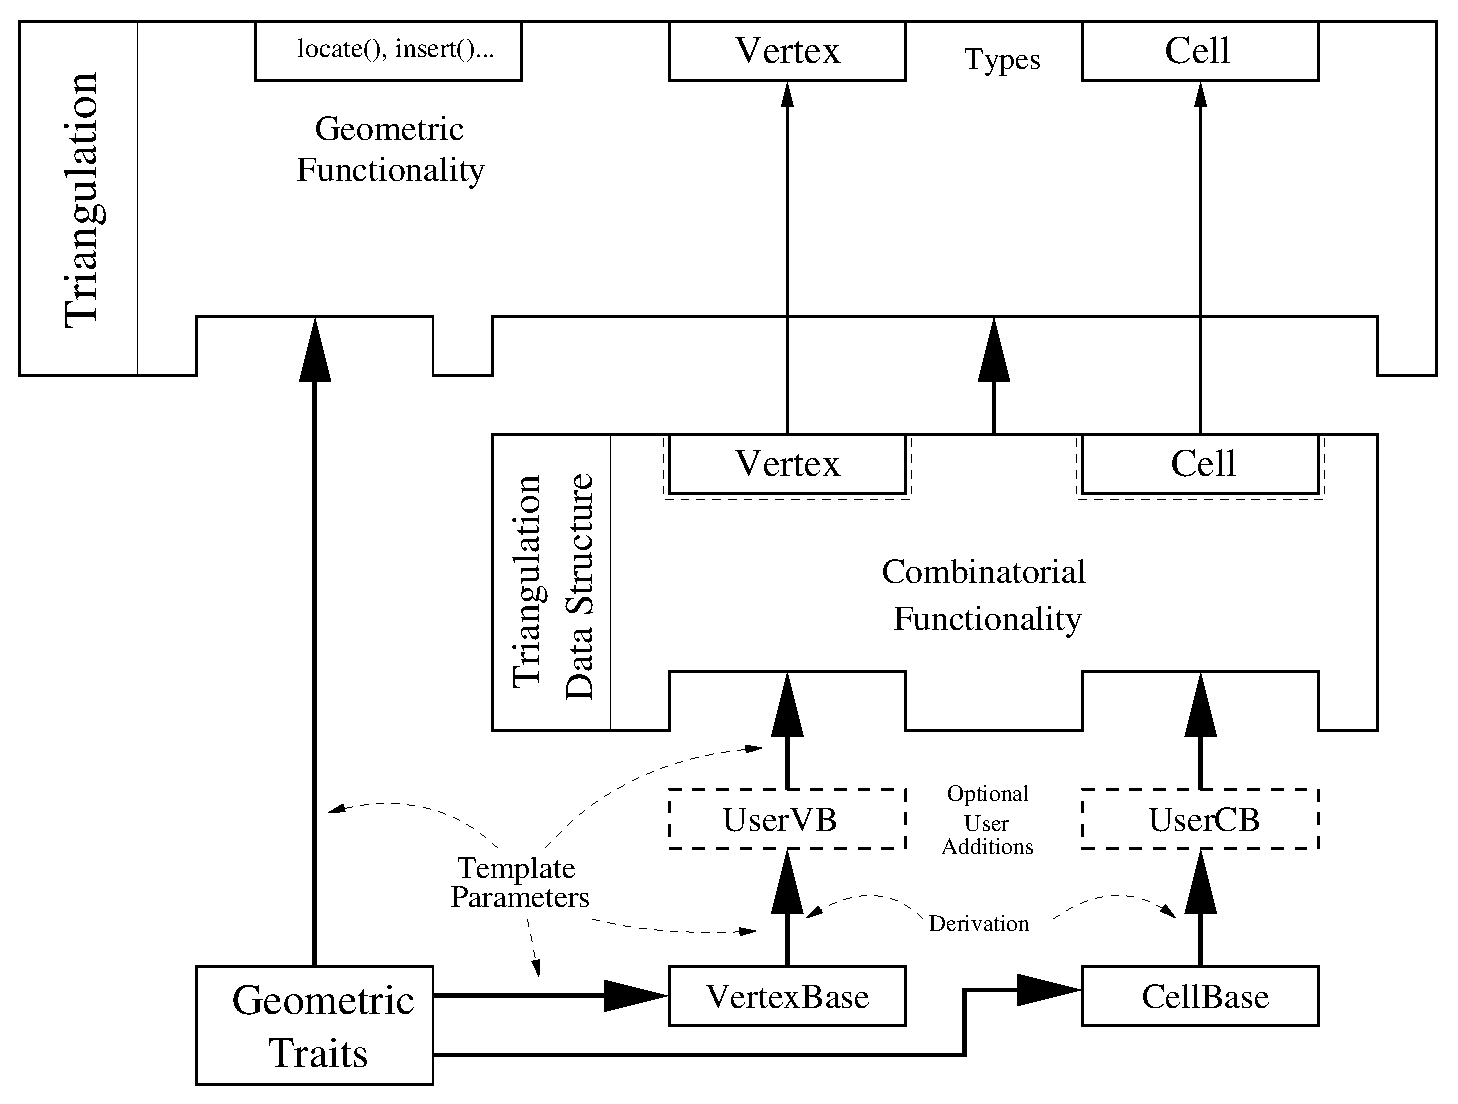
\includegraphics[width=13cm]{design.eps}
\end{center}
\end{ccTexOnly}
\caption{Triangulation software design.
\label{T3-fig-layers}}
\begin{ccHtmlOnly}
<CENTER>
<img border=0 src="./design.gif" align=center
 alt="Triangulation software design">
</CENTER>
\end{ccHtmlOnly}
\end{figure}

\subsection{Backward compatibility}
\label{T3-sec-compat}

Starting with \cgal\ release 3.0, the design of the triangulation data
structure has been changed in order to give the possibility to store handles
(an entity akeen to pointers) directly in the vertex and cell base classes.
Previously, \texttt{void*} pointers were stored there instead, and later
converted internally to handles, but this happened to be too restrictive for
some uses.

The difference is visible to the user when he provides his own vertex or cell
base class.  Previously, something like the following had to be written:

\begin{ccExampleCode}
...
template < class GT >
class My_vertex
  : public Triangulation_vertex_base<GT>
{
  typedef Triangulation_vertex_base<GT>  Vb;
public:
  typedef typename Vb::Point             Point;

  My_vertex() {}
  My_vertex(const Point&p)          : Vb(p) {}
  My_vertex(const Point&p, void *c) : Vb(p, c) {}
...
};

typedef Cartesian<double>                                               GT;
typedef Triangulation_data_structure_3<My_vertex<GT>,
                                       Triangulation_cell_base_3<GT> >  My_TDS;
typedef Triangulation_3<GT, My_TDS>                                     Tr;
...
\end{ccExampleCode}

While now, there are two possibilities.  The simplest one is to use the
class \ccc{Triangulation_vertex_base_with_info_3}, and this approach is
illustrated in a following subsection~\ref{Triangulation3-sec-examples-color}.
But when the user needs to access some type which depends on the triangulation
data structure (typically handles), then he must write:
\begin{ccExampleCode}
...
template < class GT, class Vb = Triangulation_vertex_base<GT> >
class My_vertex
  : public Vb
{
public:
  typedef typename Vb::Point           Point;
  typedef typename Vb::Cell_handle     Cell_handle;

  template < class TDS2 >
  struct Rebind_TDS {
    typedef typename Vb::template Rebind_TDS<TDS2>::Other  Vb2;
    typedef My_vertex<GT, Vb2>                             Other;
  };

  My_vertex() {}
  My_vertex(const Point&p)                : Vb(p) {}
  My_vertex(const Point&p, Cell_handle c) : Vb(p, c) {}
...
};
... // The rest has not changed
\end{ccExampleCode}

The changes that need to be made are the following:
\begin{itemize}
\item{} \ccc{My_vertex} has to be parameterized by the vertex base class it
        derives from.
\item{} a nested template class \ccc{Rebind_TDS} has to be defined.
\item{} \texttt{void*} has to be changed to \ccc{Cell_handle}, and you need to
	extract the \ccc{Cell_handle} type from the vertex base class that
        \ccc{My_vertex} derives from.
\end{itemize}

The situation is exactly similar for cell base classes.
Section~\ref{TDS3-sec-design} provides more detailed information.

\section{Examples}
\label{Triangulation3-sec-examples}
\subsection{Basic example}
This example shows the incremental construction of a 3D triangulation, the
location of a point and how to perform elementary operations on indices in a
cell. It uses the default parameter of the \ccc{Triangulation_3} class.

\ccIncludeExampleCode{Triangulation_3/example_simple.C}

\subsection{Changing the vertex base}
The following two examples show how the user can plug his own vertex base in a
triangulation.  Changing the cell base is similar.

\subsubsection{Adding a color}
\label{Triangulation3-sec-examples-color}
When the user doesn't need to add a type in a vertex which depends on the
\ccc{TriangulationDataStructure_3} (e.g. a \ccc{Vertex_handle} or
\ccc{Cell_handle}), then he can use the
\ccc{Triangulation_vertex_base_with_info_3} class to add his own information
easily in the vertices.  The example below shows how to add a \ccc{CGAL::Color}
this way.

\ccIncludeExampleCode{Triangulation_3/example_color.C}

\subsubsection{Adding handles}
When the user needs to add a type in a vertex which depends on the
\ccc{TriangulationDataStructure_3} (e.g. a \ccc{Vertex_handle} or
\ccc{Cell_handle}), then he has to derive his own vertex base class,
as the following example shows.

\ccIncludeExampleCode{Triangulation_3/example_adding_handles.C}

\subsection{Use of the Delaunay hierarchy}

\ccIncludeExampleCode{Triangulation_3/example_hierarchy.C}

\subsection{Finding the cells in conflict with a point in a Delaunay
triangulation}

\ccIncludeExampleCode{Triangulation_3/example_find_conflicts.C}
